\documentclass[svgnames]{beamer}
\mode<presentation>
\usefonttheme{serif}
\usecolortheme{dove}
\useinnertheme{rounded}
%\useoutertheme{smoothbars}
\setbeamercolor{item projected}{fg=black}
\setbeamertemplate{navigation symbols}{}

\usepackage[english]{babel}
\usepackage[latin1]{inputenc}
\usepackage{times}
\usepackage{amsthm,amssymb,amsmath,graphicx}
\usepackage{color}
\usepackage{gastex}
\usepackage{framed}
\usepackage{graphicx}
\usepackage{multicol}
\usepackage{ulem}
\usepackage{ifthen}
\usepackage{tikz}

%%%%%%%%%%%%%%%%%%%%%%%%%%%%%%%%%%%%%%%%%%%%%%%%%%%%%%%%%%%%%%%%%%%%%%%%%%%%%%%%%%%%%%%%
%%%%%%%%%%%%%%%%%%%% A non-original creation by Nathanaël Fijalkow and Victor Marsault %

\setbeamertemplate{frametitle}{
  \vskip-2pt
  \begin{beamercolorbox}[rightskip=2cm,leftskip=1em,dp=1ex,wd=12.8cm]{frametitle}
    \vskip2pt
    \usebeamercolor{frametitle}
    \begin{tikzpicture}
      \useasboundingbox (0,0) rectangle (0,0); 
      \ifthenelse{\insertframenumber<\inserttotalframenumber}
      { 
        \pgfmathsetmacro{\aimangle}{90-(\insertframenumber*360/\inserttotalframenumber)}
        \fill [fill=frametitle.fg,thin, color=gray!50,draw=black] (11.8,.2) -- (11.8,.6) arc (90:\aimangle:0.4) -- cycle;

      }{ 
        \fill[fill=frametitle.fg,thin, color=gray!50,draw=black] (11.8,0.2) circle (.4);
      }
      \fill[fill=frametitle.fg,thin, color=white,draw=black] (11.8,0.2) circle (.3);
      \node at (11.8, .2) [black,circle]{\normalsize\insertframenumber};
    \end{tikzpicture}
    \insertframetitle
    \vskip2pt
  \end{beamercolorbox}
}
%%%%%%%%%%%%%%%%%%%%%%%%%%%%%%%%%%%%%%%%%%%%%%%%%%%%%%%%%%%%%%%%%%%%%%%%%%%%%%%%%%%%%%%

\setbeamertemplate{blocks}[rounded]
\setbeamercolor{block title}{bg=normal text.bg!90!black}
\setbeamercolor{block body}{bg=normal text.bg!95!black}

\newcommand{\A}{\mathcal{A}}
\newcommand{\B}{\mathcal{B}}
\newcommand{\Q}{\mathbb{Q}}
\newcommand{\N}{\mathbb{N}}
\newcommand{\tr}[1]{\langle #1 \rangle}
\newcommand{\prob}[1]{\mathbb{P}_{#1}}
\newcommand{\set}[1]{\{ #1 \}}
\newcommand{\val}[1]{\text{val}(#1)}

  
\title{Algebraic Algorithms for Probabilistic Automata}
\subtitle{ONERA, Toulouse}
\author{Nathana\"el Fijalkow}
\institute{LIAFA, Universit\'e Denis Diderot - Paris 7, France\\
Institute of Informatics, Warsaw University, Poland}

\date{January 26th, 2015}

\AtBeginSection[]
{
\addtocounter{framenumber}{-1}
  \begin{frame}<beamer>{Outline}
    \tableofcontents[currentsection]
  \end{frame}
}

\AtBeginSubsection[]
{
\addtocounter{framenumber}{-1}
  \begin{frame}<beamer>{Outline}
    \tableofcontents[currentsection,currentsubsection]
  \end{frame}
}

\begin{document}

\addtocounter{framenumber}{-1}

\begin{frame}
  \titlepage
\end{frame}

\begin{frame}{Non-deterministic Automata}
\begin{figure}
\begin{center}
\begin{picture}(60,14)(0,0)
	\gasset{Nw=6,Nh=6,loopdiam=6}

  	\node[Nmarks=i,iangle=-90](0)(20,5){$0$}
  	\node(1)(40,5){$1$}
  	\node[Nmarks=r](F)(60,5){$F$}
  	\node(bottom)(0,5){$\perp$}

	\drawloop(0){$a$}
	\drawloop(1){$a$}
	\drawloop[loopangle=0](F){$a,b$}
	\drawloop[loopangle=180](bottom){$a,b$}

  	\drawedge(0,bottom){$b$}
  	\drawedge[curvedepth=2](0,1){$a$}
  	\drawedge[curvedepth=2](1,0){$b$}
  	\drawedge(1,F){$b$}
\end{picture}
\end{center}
\end{figure}
\vspace*{1em}

$$\tr{a} = 
\left(\begin{array}{cccc}
1 & 0 & 0 & 0 \\
0 & 1 & 1 & 0 \\
0 & 0 & 1 & 0 \\
0 & 0 & 0 & 1
\end{array}\right)
\qquad
\tr{b} = 
\left(\begin{array}{cccc}
1 & 0 & 0 & 0 \\
1 & 0 & 0 & 0 \\
0 & 1 & 0 & 1 \\
0 & 0 & 0 & 1
\end{array}\right)$$
\end{frame}

\begin{frame}{Probabilistic Automata}
\begin{figure}
\begin{center}
\begin{picture}(60,14)(0,0)
	\gasset{Nw=6,Nh=6,loopdiam=6}

  	\node[Nmarks=i,iangle=-90](0)(20,5){$0$}
  	\node(1)(40,5){$1$}
  	\node[Nmarks=r](F)(60,5){$F$}
  	\node(bottom)(0,5){$\perp$}

	\drawloop(0){$a:0.5$}
	\drawloop(1){$a$}
	\drawloop[loopangle=0](F){$a,b$}
	\drawloop[loopangle=180](bottom){$a,b$}

  	\drawedge(0,bottom){$b$}
  	\drawedge[curvedepth=2](0,1){$a:0.5$}
  	\drawedge[curvedepth=2](1,0){$b:0.7$}
  	\drawedge(1,F){$b:0.3$}
\end{picture}
\end{center}
\end{figure}
\vspace*{1em}

$$\tr{a} = 
\left(\begin{array}{cccc}
1 & 0 & 0 & 0 \\
0 & 0.5 & 0.5 & 0 \\
0 & 0 & 1 & 0 \\
0 & 0 & 0 & 1
\end{array}\right)
\qquad
\tr{b} = 
\left(\begin{array}{cccc}
1 & 0 & 0 & 0 \\
1 & 0 & 0 & 0 \\
0 & 0.7 & 0 & 0.3 \\
0 & 0 & 0 & 1
\end{array}\right)$$
\end{frame}

\begin{frame}{Computing with Matrices}

Let $u = abaaba$.

$$\prob{\A}(u) = I \cdot \underbrace{\tr{a} \cdot \tr{b} \cdot \tr{a} \cdot \tr{a} \cdot \tr{b} \cdot \tr{a}}_{\tr{u}} \cdot F$$

\vskip2em
\begin{center}
\begin{huge}
Everything boils down to\\[0.6em]
matrix multiplications!
\end{huge}
\end{center}
\end{frame}

\begin{frame}{Algorithmic Properties of Probabilistic Automata}
$$L^{> \frac{1}{2}}(\A) = \set{w \in A^* \mid \prob{\A}(w) > \frac{1}{2}}$$
\begin{enumerate}
	\item \textit{Emptiness}: $L^{> \frac{1}{2}}(\A) = \emptyset$?
	\item \textit{Universality}: $L^{> \frac{1}{2}}(\A) = A^*$?
	\item \textit{Equivalence}: is it true that for all words $w \in A^*$, we have $\prob{\A}(w) = \prob{\B}(w)$?
	\item \textit{Regularity}: is the language $L^{> \frac{1}{2}}(\A) = $ regular?
	\item \textit{Value}: is the value $\val{\A} = \sup_{w \in A^*} \prob{\A}(w)$ computable? Approximable?
	\item \textit{Value 1}: is it true that $\val{\A} = 1$?	
\end{enumerate}
\vskip1em
\pause
\begin{center}
\begin{huge}
We would like to finitely represent\\[0.6em]
$\set{\tr{w} \mid w \in A^*}$
\end{huge}
\end{center}
\end{frame}

\begin{frame}{Negative Results}
\begin{theorem}[Results from 1963 to 2010]
\begin{itemize}
	\item The Emptiness, Universality, Regularity and Value $1$ problems are undecidable.
	\item The Value cannot be computed, nor approximated, even up to the constant $\frac{1}{6}$.
\end{itemize}
\end{theorem}
\vskip2em
\pause
\begin{center}
\begin{huge}
It is hard to accurately represent\\[0.6em]
$\set{\tr{w} \mid w \in A^*}$
\end{huge}
\end{center}
\end{frame}

\begin{frame}{Positive Results}
\begin{theorem}[Sch\"utzenberg 61]
The Equivalence problem is decidable in polynomial time.
\end{theorem}
Indeed:
$$\begin{array}{c}
\forall w \in A^*,\quad \prob{\A}(w) = \prob{\B}(w) \\[.6em]
\Longleftrightarrow \\[.6em]
\forall w \in A^{\le |\A| + |\B|},\quad \prob{\A}(w) = \prob{\B}(w)
\end{array}$$
\pause

\begin{center}
$\looparrowright$
The best (randomized) algorithm is to pick small words\\
at random and to check the equality.
\end{center}
\end{frame}

\begin{frame}{The Value $1$ Problem}
\begin{center}
Is the value $\val{\A} = \sup_{w \in A^*} \prob{\A}(w)$ equal to $1$?
\end{center}

Equivalently:	
\begin{center}
Is it true that for all $\varepsilon > 0$, \\
there exists $w \in A^*$ such that $\prob{\A}(w) \ge 1 - \varepsilon$?
\end{center}

\pause
\vskip2em
\begin{center}
\begin{huge}
This is undecidable,\\[.6em]
but we can construct an algorithm\\[.6em]
which is \textit{often} correct!
\end{huge}
\end{center}
\end{frame}

\begin{frame}{\ }
\begin{center}
\begin{Huge}
The virtues of the\\[1em]
Markov Monoid algorithm
\end{Huge}
\end{center}
\end{frame}

\begin{frame}{No numerical values}
\begin{figure}
\begin{center}
\begin{picture}(60,14)(0,0)
	\gasset{Nw=6,Nh=6,loopdiam=6}

  	\node[Nmarks=i,iangle=-90](0)(20,5){$0$}
  	\node(1)(40,5){$1$}
  	\node[Nmarks=r](F)(60,5){$F$}
  	\node(bottom)(0,5){$\perp$}

	\drawloop(0){$a:0.5$}
	\drawloop(1){$a$}
	\drawloop[loopangle=0](F){$a,b$}
	\drawloop[loopangle=180](bottom){$a,b$}

  	\drawedge(0,bottom){$b$}
  	\drawedge[curvedepth=2](0,1){$a:0.5$}
  	\drawedge[curvedepth=2](1,0){$b:0.7$}
  	\drawedge(1,F){$b:0.3$}
\end{picture}
\end{center}
\end{figure}
\begin{Huge}$$\Downarrow$$\end{Huge}
\begin{figure}
\begin{center}
\begin{picture}(60,14)(0,0)
	\gasset{Nw=6,Nh=6,loopdiam=6}

  	\node[Nmarks=i,iangle=-90](0)(20,5){$0$}
  	\node(1)(40,5){$1$}
  	\node[Nmarks=r](F)(60,5){$F$}
  	\node(bottom)(0,5){$\perp$}

	\drawloop(0){$a$}
	\drawloop(1){$a$}
	\drawloop[loopangle=0](F){$a,b$}
	\drawloop[loopangle=180](bottom){$a,b$}

  	\drawedge(0,bottom){$b$}
  	\drawedge[curvedepth=2](0,1){$a$}
  	\drawedge[curvedepth=2](1,0){$b$}
  	\drawedge(1,F){$b$}
\end{picture}
\end{center}
\end{figure}
\end{frame}

\begin{frame}{An example}
\begin{figure}
\begin{center}
\begin{picture}(60,15)(0,-5)
	\gasset{Nw=6,Nh=6,loopdiam=6}

  	\node[Nmarks=i,iangle=-90](0)(20,5){$0$}
  	\node(1)(40,5){$1$}
  	\node[Nmarks=r](F)(60,5){$F$}
  	\node(bottom)(0,5){$\perp$}

	\drawloop(0){$a$}
	\drawloop(1){$a$}
	\drawloop[loopangle=0](F){$a,b$}
	\drawloop[loopangle=180](bottom){$a,b$}

  	\drawedge(0,bottom){$b$}
  	\drawedge[curvedepth=2](0,1){$a$}
  	\drawedge[curvedepth=2](1,0){$b$}
  	\drawedge(1,F){$b$}
\end{picture}
\pause
\begin{picture}(60,10)(0,0)
	\gasset{Nw=5,Nh=5,loopdiam=4}

	\put(-20,4){$\tr{a}$}

  	\node(0)(20,5){$0$}
  	\node(1)(40,5){$1$}
  	\node[Nmarks=r](F)(60,5){$F$}
  	\node(bottom)(0,5){$\perp$}

	\drawloop(0){}
	\drawloop(1){}
	\drawloop[loopangle=0](F){}
	\drawloop[loopangle=180](bottom){}

  	\drawedge(0,1){}
\end{picture}
\pause
\begin{picture}(60,10)(0,0)
	\gasset{Nw=5,Nh=5,loopdiam=4}

	\put(-20,4){$\tr{b}$}

  	\node(0)(20,5){$0$}
  	\node(1)(40,5){$1$}
  	\node[Nmarks=r](F)(60,5){$F$}
  	\node(bottom)(0,5){$\perp$}

	\drawloop[loopangle=0](F){}
	\drawloop[loopangle=180](bottom){}

  	\drawedge(0,bottom){}
  	\drawedge(1,0){}
  	\drawedge(1,F){}
\end{picture}
\pause
\begin{picture}(60,10)(0,0)
	\gasset{Nw=5,Nh=5,loopdiam=4}

	\put(-20,4){$\tr{a^\sharp}$}

  	\node(0)(20,5){$0$}
  	\node(1)(40,5){$1$}
  	\node[Nmarks=r](F)(60,5){$F$}
  	\node(bottom)(0,5){$\perp$}

	\drawloop(1){}
	\drawloop[loopangle=0](F){}
	\drawloop[loopangle=180](bottom){}

  	\drawedge(0,1){}
\end{picture}
\pause
\begin{picture}(60,10)(0,0)
	\gasset{Nw=5,Nh=5,loopdiam=4}

	\put(-22,4){$\tr{a^\sharp \cdot b}$}

  	\node(0)(20,5){$0$}
  	\node(1)(40,5){$1$}
  	\node[Nmarks=r](F)(60,5){$F$}
  	\node(bottom)(0,5){$\perp$}

	\drawloop(0){}
	\drawloop[loopangle=0](F){}
	\drawloop[loopangle=180](bottom){}

  	\drawedge[curvedepth=-4](0,F){}
  	\drawedge(1,0){}
  	\drawedge(1,F){}
\end{picture}
\pause
\begin{picture}(60,10)(0,0)
	\gasset{Nw=5,Nh=5,loopdiam=4}

	\put(-25,4){$\tr{(a^\sharp \cdot b)^\sharp}$}

  	\node(0)(20,5){$0$}
  	\node(1)(40,5){$1$}
  	\node[Nmarks=r](F)(60,5){$F$}
  	\node(bottom)(0,5){$\perp$}

	\drawloop[loopangle=0](F){}
	\drawloop[loopangle=180](bottom){}

  	\drawedge[curvedepth=-4](0,F){}
  	\drawedge(1,F){}
\end{picture}
\end{center}
\end{figure}
\end{frame}

\begin{frame}{Defining stabilization}
\begin{figure}
\begin{center}
\begin{picture}(20,10)(0,0)
	\gasset{Nw=6,Nh=6}

  	\node[Nmarks=i,iangle=180](1)(0,5){$1$}
  	\node[Nmarks=r](2)(20,5){$2$}

	\drawloop(1){$a$}
  	\drawedge(1,2){$a$}
	\drawloop(2){$a$}
\end{picture}
\end{center}
\end{figure}

$$\tr{a} = 
\left(\begin{array}{ccc}
1 & 1 \\
0 & 1
\end{array}\right)
\qquad
\only<2,3>{
\tr{a^\sharp} = 
\left(\begin{array}{ccc}
0 & 1\\
0 & 1
\end{array}\right)}$$

In $\tr{a}$, the state $1$ is transient and the state $2$ is recurrent.

\only<3>{
$$M^\sharp(s,t) = 
\left\{\begin{array}{ll}
1 & \textrm{if } M(s,t) = 1 \textrm{ and } t \textrm{ recurrent in } M,\\
0 & \textrm{otherwise.}
\end{array}\right.$$
}
\end{frame}

\begin{frame}{Markov Monoid of an Automaton}
\begin{center}
Matrix multiplication $\longleftrightarrow$ concatenation

\pause
\vskip2em
Stabilization $\longleftrightarrow$ limit of the powers
\vskip1em
$\tr{u}^\sharp$ represents $\lim_n \tr{u^n}$
\end{center}

\pause
\begin{definition}
The Markov Monoid of $\A$ is the closure of $\set{\tr{a} \mid a \in A}$ under multiplication and stabilization.
\end{definition}

\vskip1em
The Markov Monoid of $\A$ contains a lot of information about $\A$!
\end{frame}

\begin{frame}{Value $1$ Witnesses}
\begin{definition} $M$ is a value $1$ witness if
$$\forall t \in Q, \quad M(s_0,t) = 1 \Rightarrow t \in F$$
\end{definition}
\vskip2em
\begin{center}
If there exists a value $1$ witness,\\
then the algorithm answers ``$\A$ has value $1$'',\\
otherwise ``$\A$ does not have value $1$''.
\end{center}
\end{frame}

\begin{frame}{Correctness}
\begin{theorem}
If there exists a value $1$ witness, then $\A$ has value $1$.
\end{theorem}
\pause
But the value $1$ problem is undecidable, so\ldots
\end{frame}

\begin{frame}{No completeness}
\only<1>{
\begin{center}
\begin{picture}(100,50)(0,0)
	\gasset{Nadjust=wh,Nadjustdist=2,fillcolor=Gray!50}

  	\node[Nmarks=i,iangle=235](H1)(0,30){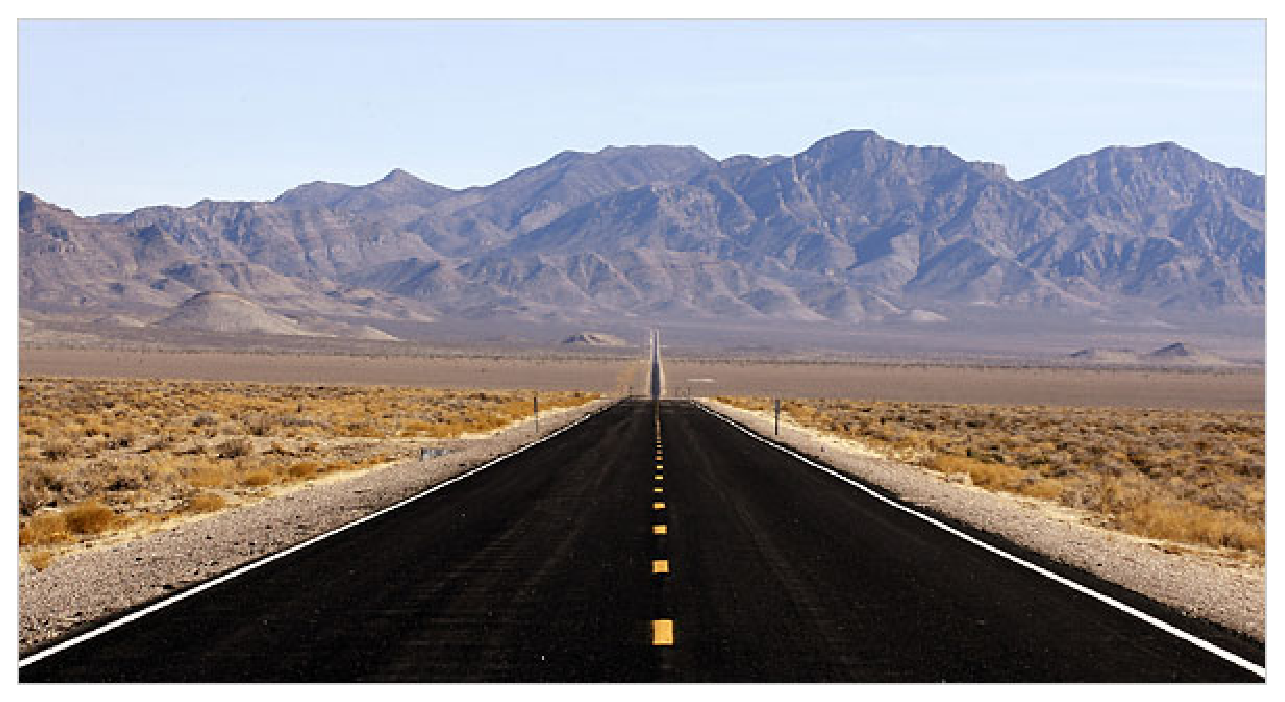
\includegraphics[scale=.1]{high.eps}}
  	\node[linecolor=White](H1)(0,30){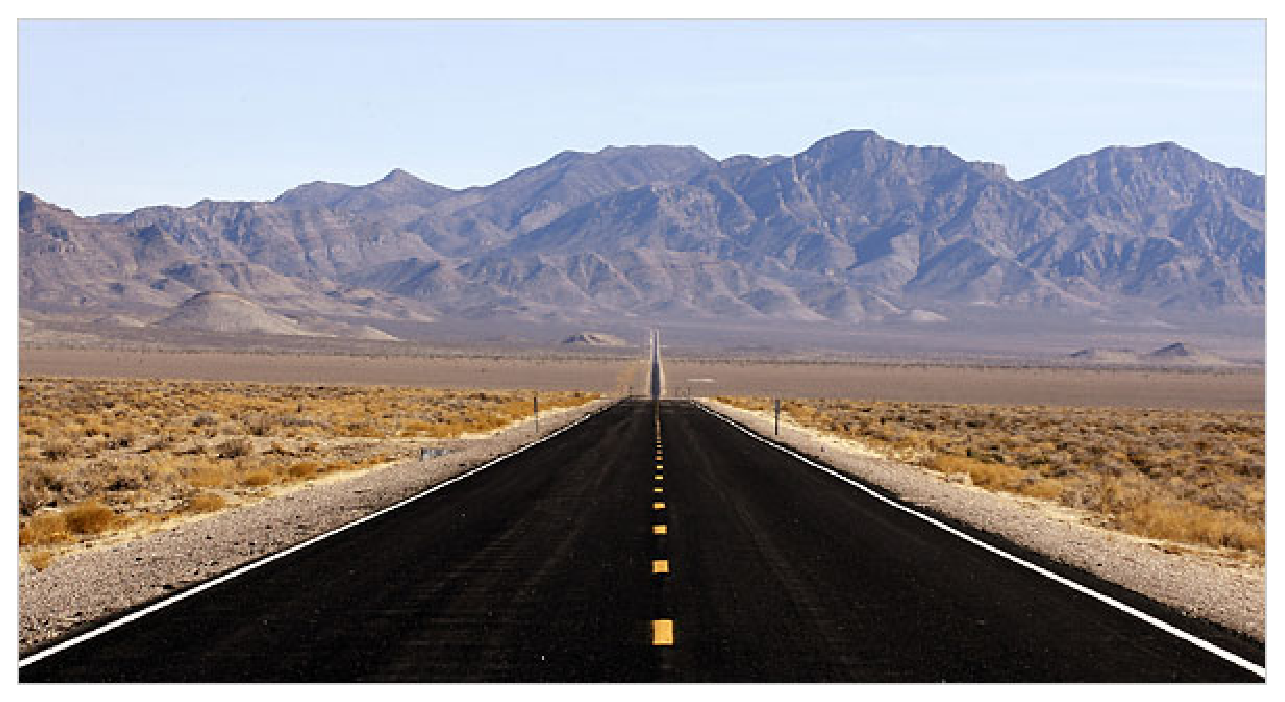
\includegraphics[scale=.1]{high.eps}}
  	\node[linecolor=White](H2)(50,30){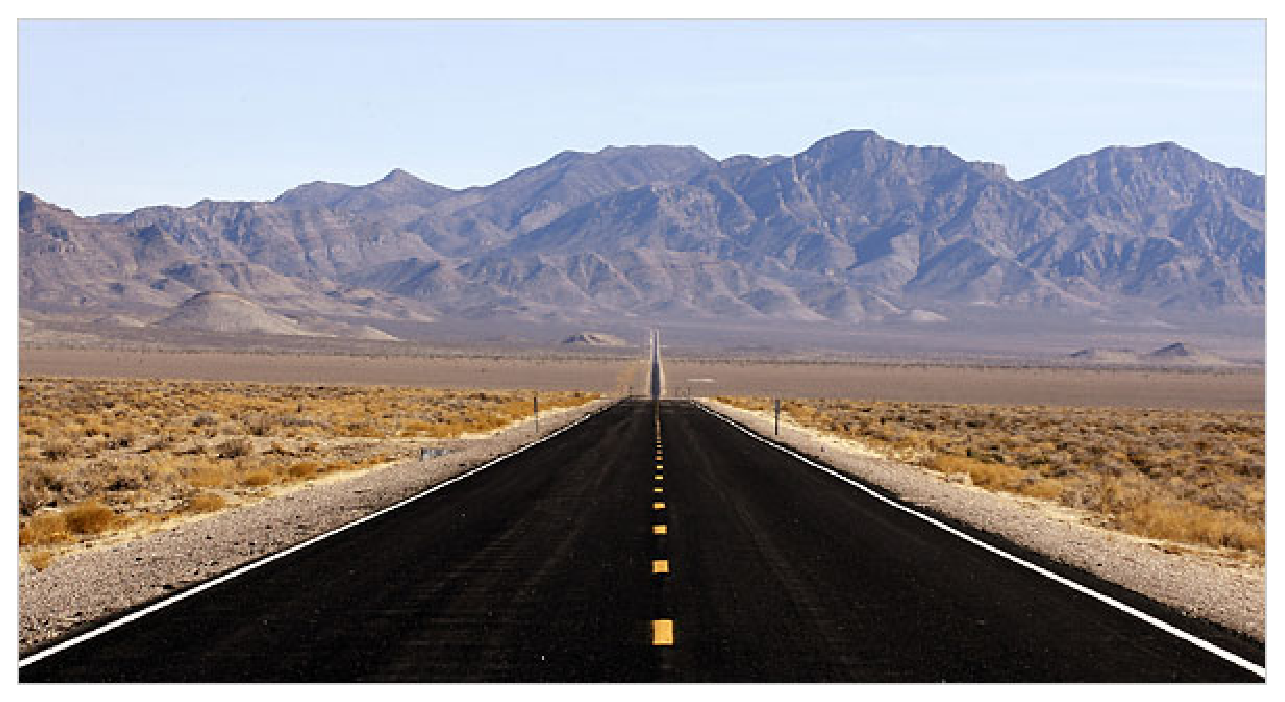
\includegraphics[scale=.1]{high.eps}}
  	\node[linecolor=White](H3)(100,30){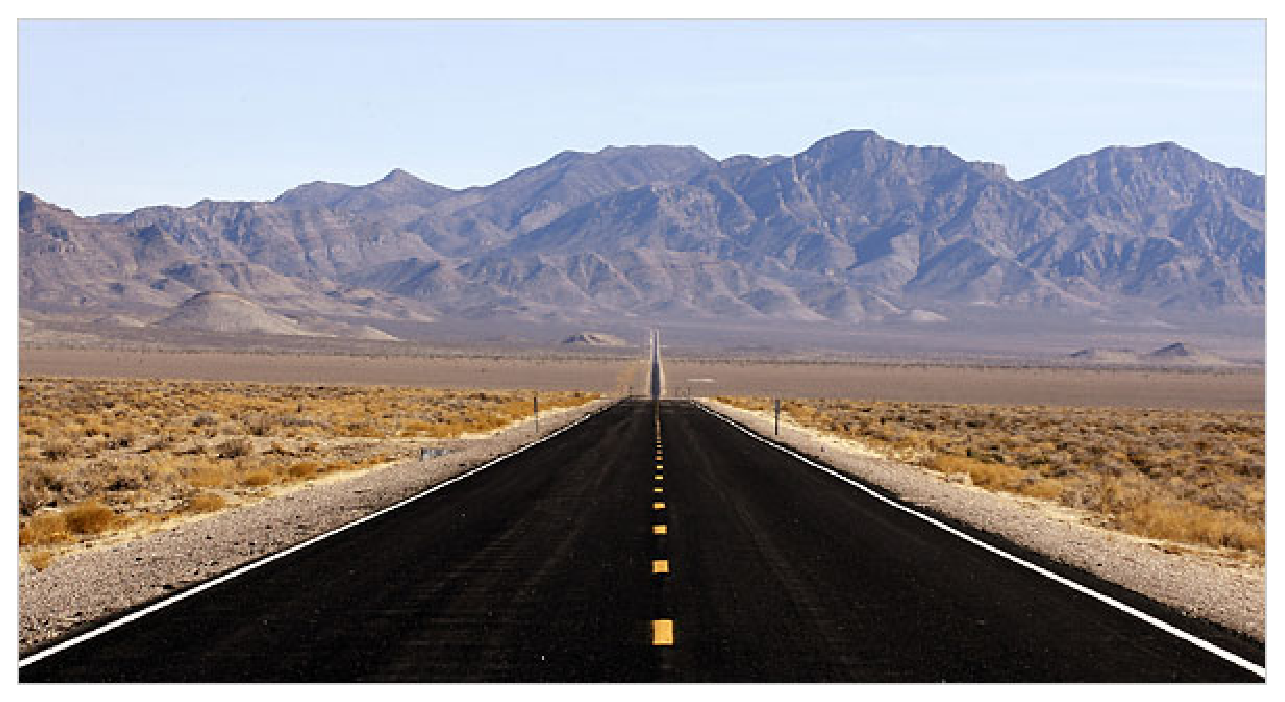
\includegraphics[scale=.1]{high.eps}}
  	\node[linecolor=White](N)(25,0){
\includegraphics[scale=.18]{lost.eps}}
  	\node[linecolor=White](C)(75,0){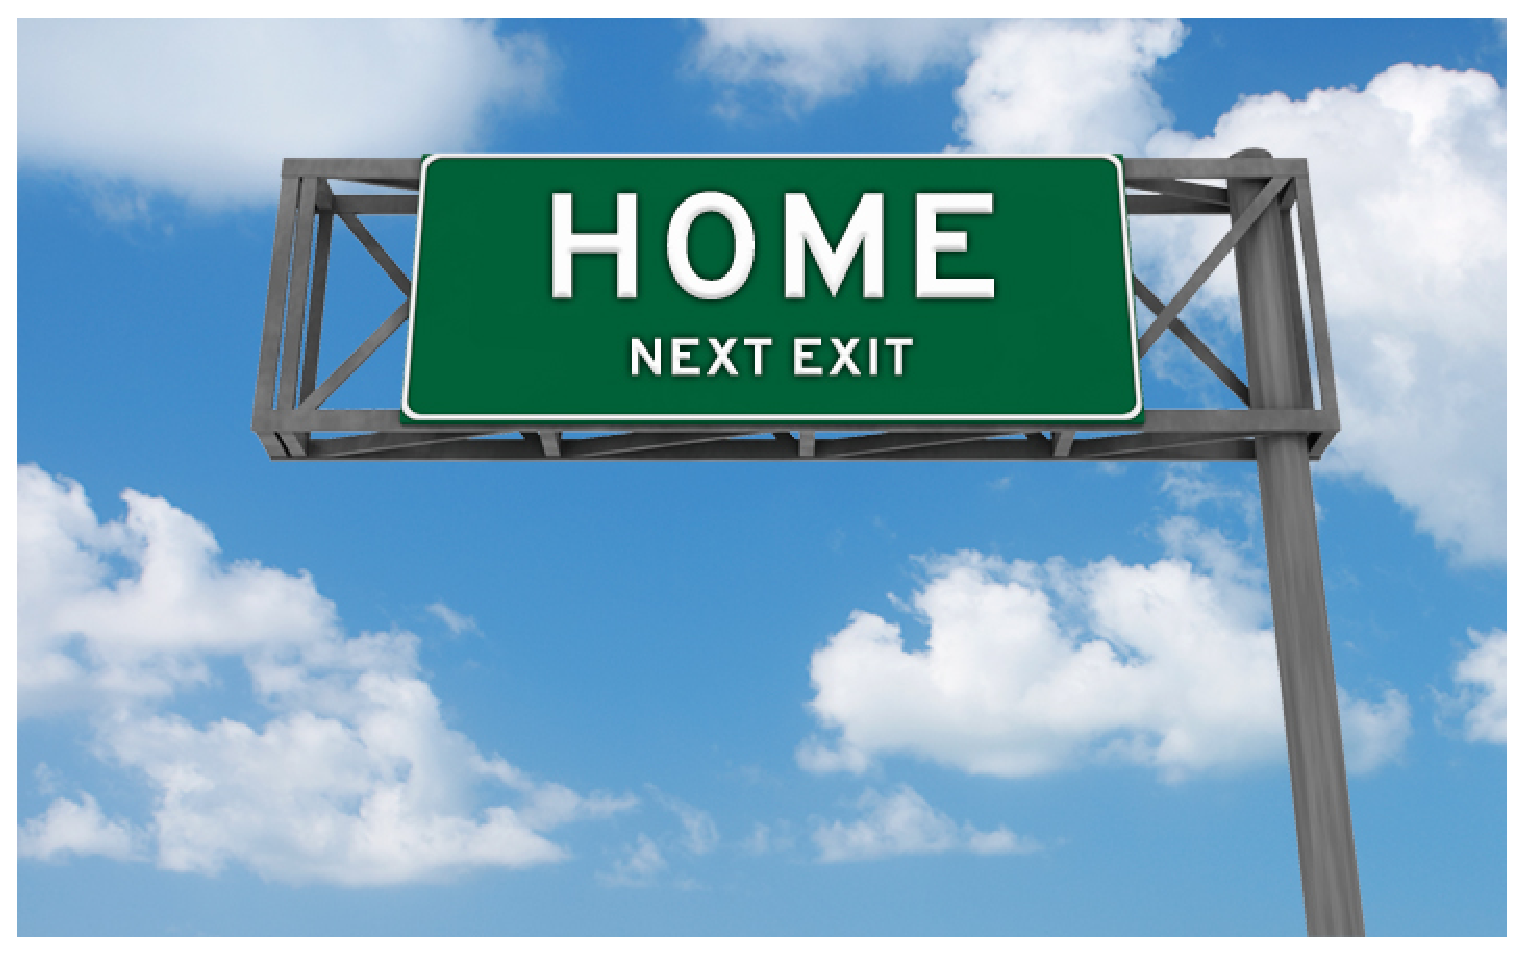
\includegraphics[scale=.1]{home.eps}}

  	\drawedge(H1,H2){$\textrm{drive}:0.6$}
  	\drawedge(H2,H3){$\textrm{drive}:0.55$}
  	\drawedge[curvedepth=-30](H3,H1){$\textrm{exit}$}
	\drawloop[loopangle=90](H1){$\textrm{drive}:0.4$}
	\drawloop[loopangle=90](H2){$\textrm{drive}:0.45$}
	\drawloop[loopangle=90](H3){$\textrm{drive}$}
  	\drawedge[curvedepth=-5](H1,N){$\textrm{exit}$}
  	\drawedge[curvedepth=-5](H2,C){$\textrm{exit}$}
	\drawloop[loopangle=180](N){}
	\drawloop[loopangle=180](C){}
\end{picture}
\end{center}
}
\only<2>{
\begin{columns}[t]
\begin{column}{0.5\textwidth}
\begin{center}
\scalebox{.5}{
\begin{picture}(100,50)(0,0)
	\gasset{Nadjust=wh,Nadjustdist=2,fillcolor=Gray!50}

  	\node[Nmarks=i,iangle=235](H1)(0,30){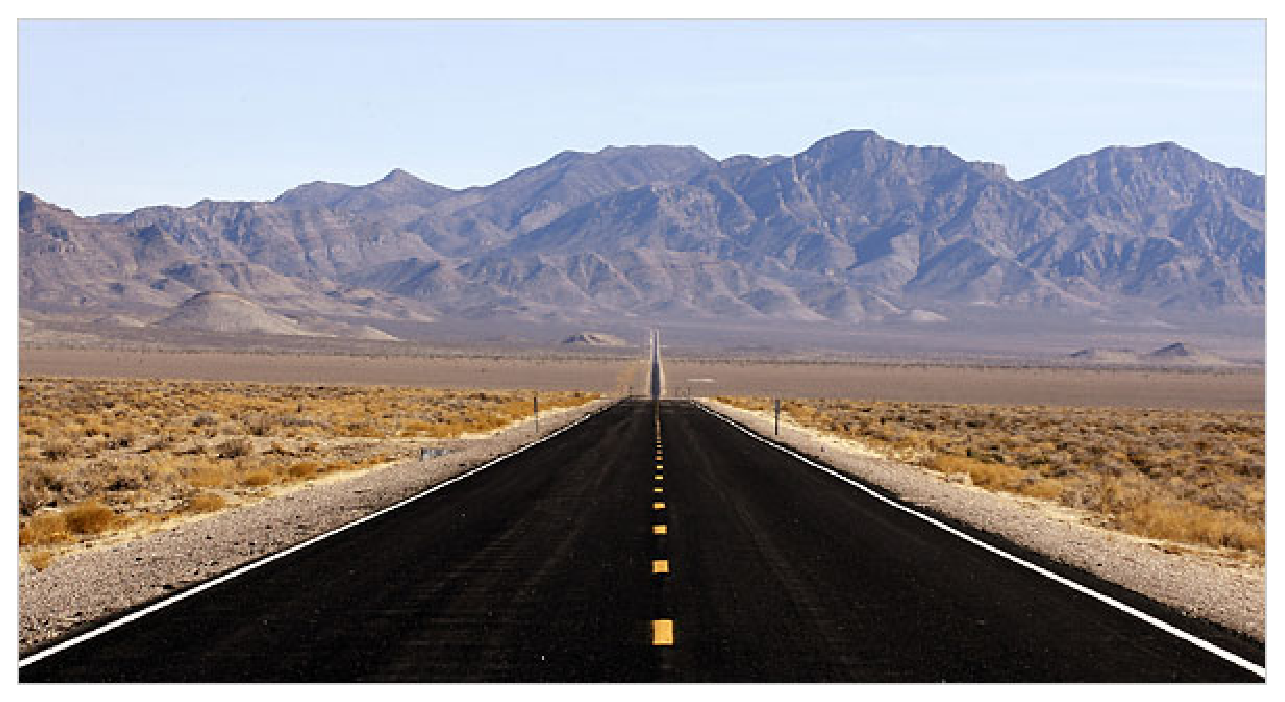
\includegraphics[scale=.1]{high.eps}}
  	\node[linecolor=White](H1)(0,30){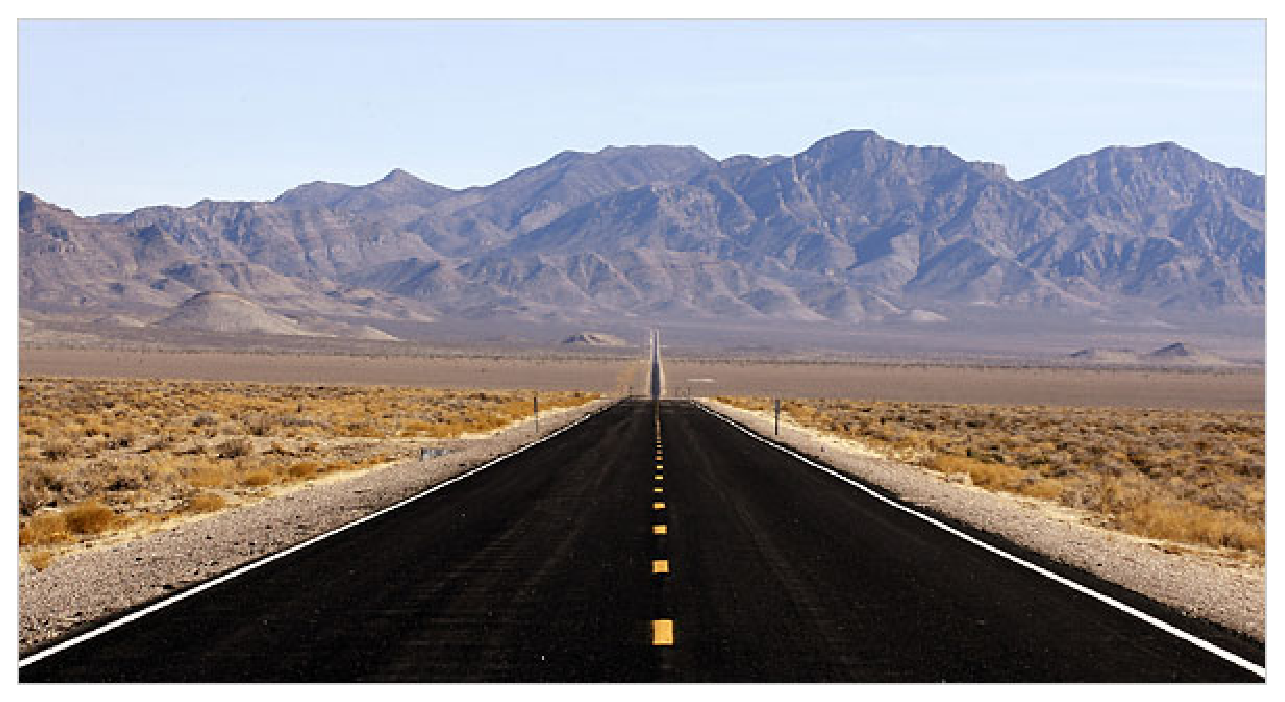
\includegraphics[scale=.1]{high.eps}}
  	\node[linecolor=White](H2)(50,30){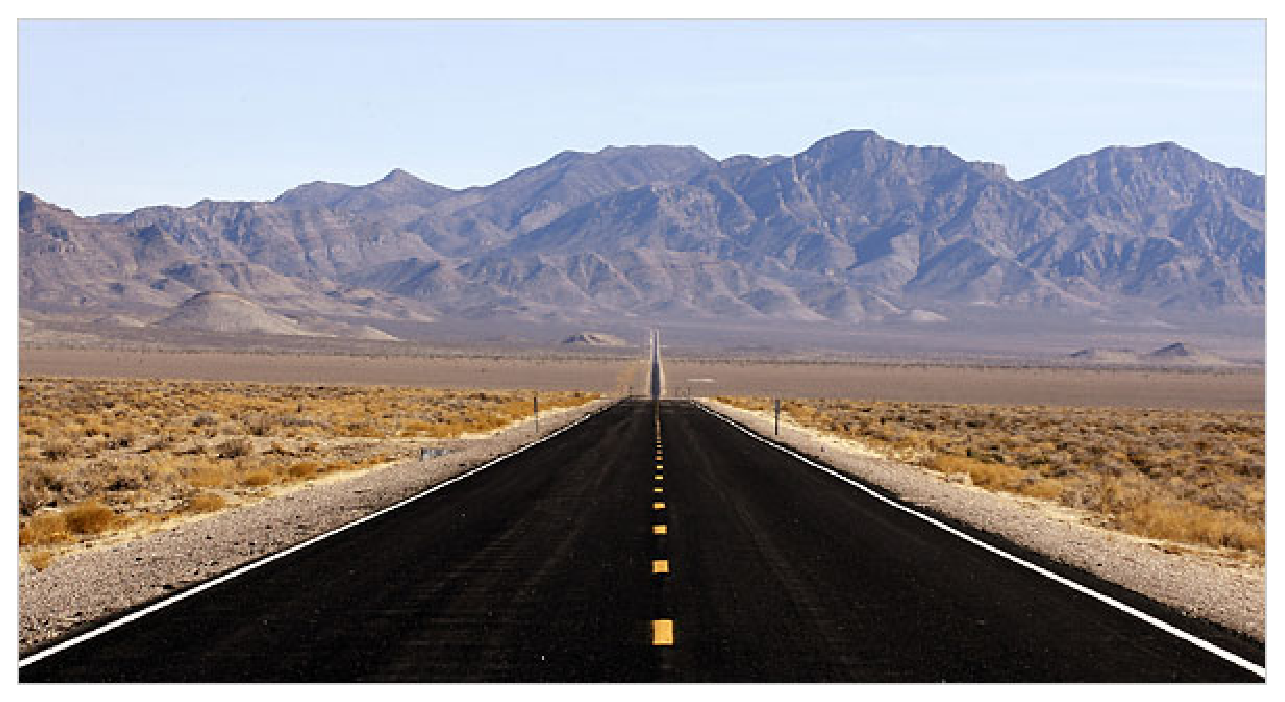
\includegraphics[scale=.1]{high.eps}}
  	\node[linecolor=White](H3)(100,30){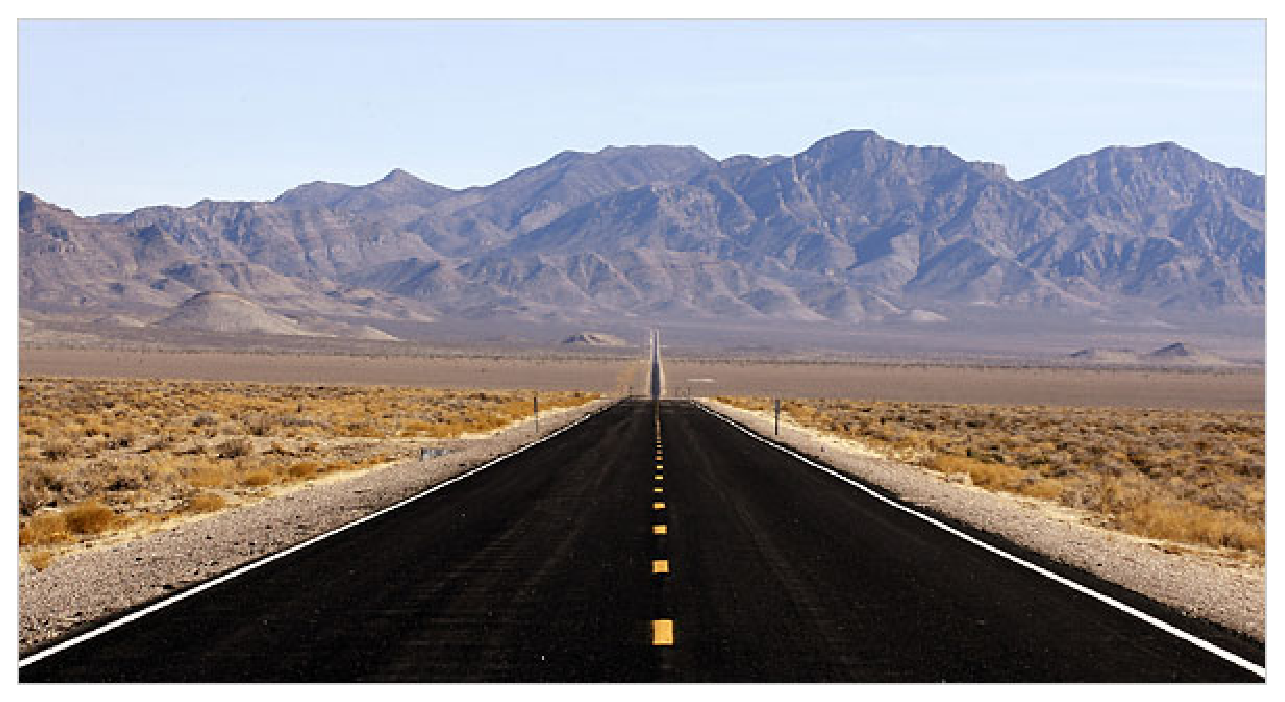
\includegraphics[scale=.1]{high.eps}}
  	\node[linecolor=White](N)(25,0){
\includegraphics[scale=.18]{lost.eps}}
  	\node[linecolor=White](C)(75,0){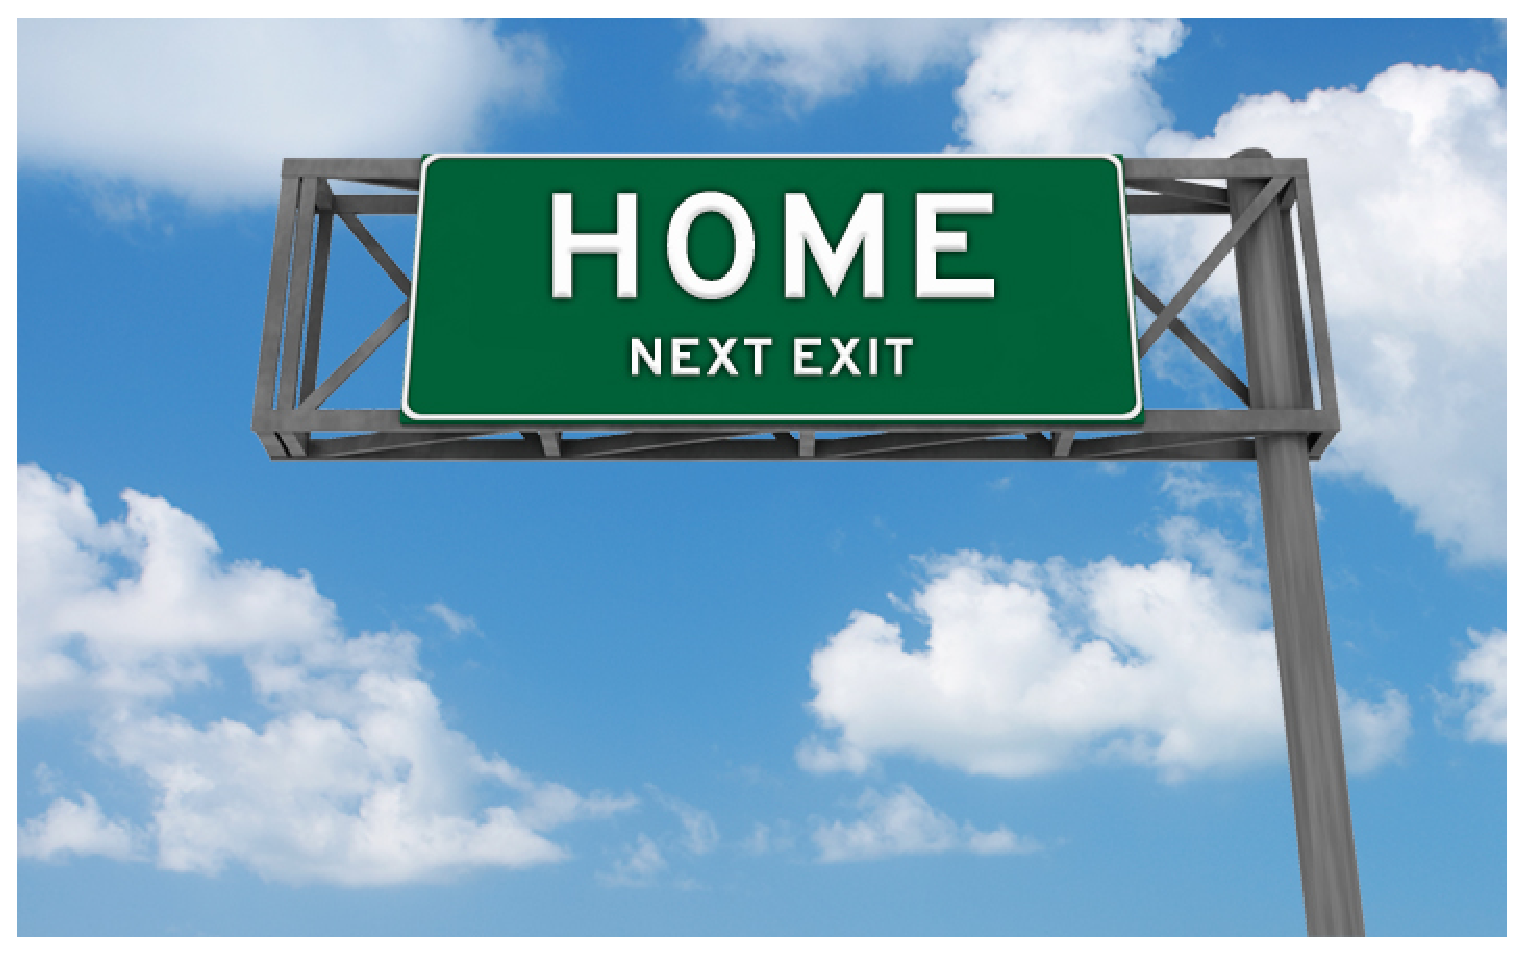
\includegraphics[scale=.1]{home.eps}}

  	\drawedge(H1,H2){$\textrm{drive}:0.6$}
  	\drawedge(H2,H3){$\textrm{drive}:0.55$}
  	\drawedge[curvedepth=-30](H3,H1){$\textrm{exit}$}
	\drawloop[loopangle=90](H1){$\textrm{drive}:0.4$}
	\drawloop[loopangle=90](H2){$\textrm{drive}:0.45$}
	\drawloop[loopangle=90](H3){$\textrm{drive}$}
  	\drawedge[curvedepth=-5](H1,N){$\textrm{exit}$}
  	\drawedge[curvedepth=-5](H2,C){$\textrm{exit}$}
	\drawloop[loopangle=180](N){}
	\drawloop[loopangle=180](C){}
\end{picture}
}
\end{center}
\end{column}
\begin{column}{0.5\textwidth}
\begin{itemize}
	\item No word ensures to reach home \textcolor{red}{\textit{almost surely}}.
	\item For every $\varepsilon > 0$, there exists a word ensuring to reach home
with probability at least $1 - \varepsilon$!
	\item This is not true anymore if the probabilities change,
	but the Markov Monoid algorithm cannot detect this!
\end{itemize}
\end{column}
\end{columns}
}
\end{frame}

%\begin{frame}{No completeness}
%\begin{figure}
%\begin{center}
%\begin{picture}(60,35)(0,0)
%	\gasset{Nw=7,Nh=7}
%
%  	\node[Nmarks=i,iangle=-90](0)(30,15){$0$}
%  	\node(L1)(0,10){$L_1$}
%  	\node[Nmarks=r](L2)(0,30){$L_2$}
%  	\node(R1)(60,10){$R_1$}
%  	\node(R2)(60,30){$R_2$}
%
%	\drawloop(0){$a$}
%
%  	\drawedge[curvedepth=5,ELside=l](0,L1){$b,\frac{1}{2}$}
%  	\drawedge[curvedepth=5,ELside=l](L1,0){$a,1-x$}
%  	\drawedge(L1,L2){$b$}
%	\drawloop[loopangle=-135](L1){$a,x$}
%	\drawloop[loopangle=90](L2){$a,b$}
%
%  	\drawedge[curvedepth=-5,ELside=r](0,R1){$b,\frac{1}{2}$}
%  	\drawedge[curvedepth=-5,ELside=r](R1,0){$a,x$}
%  	\drawedge[ELside=r](R1,R2){$b$}
%	\drawloop[loopangle=-45](R1){$a,1-x$}
%	\drawloop(R2){$a,b$}
%\end{picture}
%\end{center}
%\end{figure}
%
%Left and right parts are symmetric, so for all $M$:
%$$M(0,L_2) = 1 \Longleftrightarrow M(0,R_2) = 1.$$
%\end{frame}

\begin{frame}{Theoretical Results}
\begin{columns}[t]
\begin{column}{0.6\textwidth}
\begin{center}
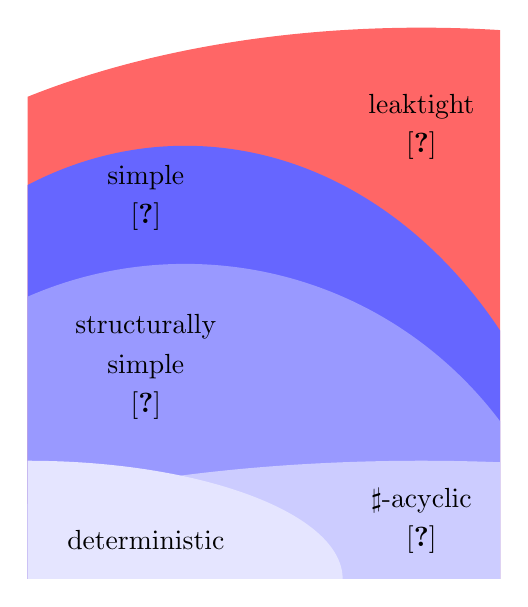
\begin{tikzpicture}
\clip (-6,2) rectangle (0,9);

\fill[red!60] (-1,5) ellipse (8cm and 4cm) ;
\draw (-1,8) node {leaktight} ;
\draw (-1,7.5) node {\cite{FGO12}} ;

\fill[blue!60] (-4,1) ellipse (5.2cm and 6.5cm) ;
\draw (-4.5,7.1) node {simple} ;
\draw (-4.5,6.6) node {\cite{CT12}} ;

\fill[blue!40] (-4,1) ellipse (5cm and 5cm) ;
\draw (-4.5,5.2) node {structurally} ;
\draw (-4.5,4.7) node {simple} ;
\draw (-4.5,4.2) node {\cite{CT12}} ;

\fill[blue!20] (-1,1) ellipse (8cm and 2.5cm) ;
\draw (-1,3) node {$\sharp$-acyclic} ;
\draw (-1,2.5) node {\cite{GO10}} ;

\fill[blue!10] (-6,2) ellipse (4cm and 1.5cm) ;
\draw (-4.5,2.5) node {deterministic} ;
\end{tikzpicture}
\end{center}
\end{column}
\begin{column}{0.5\textwidth}
\pause
In \cite{FGO12},
we introduced the Markov Monoid,
generalizing the transition monoid.
\vskip1em
\begin{theorem}[\cite{FGO12}]
The value $1$ problem is decidable for leaktight automata.
\end{theorem}
\begin{theorem}[\cite{FGKO14}]
Leaktight automata strictly contain the simple automata.
\end{theorem}
\begin{theorem}[\cite{F15}]
\textcolor{red}{The Markov Monoid algorithm is \textit{optimal}.}
\end{theorem}
\end{column}
\end{columns}
\end{frame}

\begin{frame}{Optimality Argument}
\begin{figure}
\begin{center}
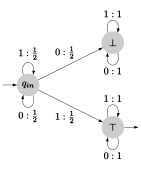
\includegraphics[scale=.7]{fig3}
\end{center}
\end{figure}
\end{frame}

\begin{frame}{MMA in Practice!}
Two implementations:
\begin{itemize}
	\item ACM\'E: a na\"ive one, written in OCaML with Denis Kuperberg,
	\item ACM\'E++: an optimized one, written in C++ with Hugo Gimbert, Edon Kelmendis and Denis Kuperberg.
\end{itemize}
\begin{figure}
\begin{center}

\includegraphics[scale=.1]{acme}
\end{center}
\end{figure}
\end{frame}

\begin{frame}{The end.}
Thank you for your attention!
\end{frame}

\begin{tiny}
\bibliographystyle{alpha}
\bibliography{bib}
\end{tiny}

\end{document}
